\documentclass[11pt]{article}
\usepackage[margin=1.05in]{geometry}
\usepackage{booktabs}
\usepackage{amsmath}
\usepackage[T1]{fontenc}
\usepackage{lmodern}
\usepackage{microtype}
\usepackage{graphicx}
\usepackage[hidelinks]{hyperref}
\usepackage{caption}
\captionsetup{font=small}

\title{Ancestry instrumentation for \texttt{fmix}}
\author{Why the origin-based transport meters stopped working,\\
what replaced them, and what the replacement measured}
\date{28 July 2026}

\begin{document}
\maketitle

\noindent Figures: \texttt{reports/ancestry\_20260728/}.

\section{The meters that broke}

\texttt{fmix} has carried three positional-mixing meters since the
directional-walk work: \texttt{odiff} (per-origin-family spread), \texttt{oadj}
(adjacent-origin autocorrelation) and \texttt{disp} (mean normalised
displacement). All three read the per-gate \texttt{origin} tag, the index of the
input gate a gate descends from.

On the restructured menu they all read ``nothing has moved'':
$\texttt{odiff}=0.0001$, $\texttt{oadj}=1.0000$ after 40M moves and
$2.58\times$ growth. Taken at face value that says the circuit is still, in
ancestry layout, the original gate order.

It does not say that. A DB splice over a window spanning \emph{mixed lineage}
stamps its products \texttt{ORIGIN\_SYNTH}, and all three statistics
\emph{skip} such gates. They are therefore computed over the material mixing has
\emph{failed to touch}, and they grow more selective the better the mixing
works---survivorship bias pointing exactly the wrong way.

\texttt{osyn} was added to make the bias visible rather than arguable. It is the
fraction of gates whose ancestry label has been destroyed:

\begin{center}
\begin{tabular}{lccccc}
\toprule
moves & 250k & 1M & 1.75M & 2.5M & 3M \\
\midrule
\texttt{osyn} & 22.9\% & \textbf{50.7\%} & 63.3\% & 72.3\% & \textbf{77.0\%} \\
\bottomrule
\end{tabular}
\end{center}

Half the circuit by 1M moves; on the small-circuit runs below it reaches
$1.000$, so there the three origin meters are not degraded but \emph{undefined}.

\paragraph{Rule.} Read \texttt{osyn} first. Once it is high, the origin meters
carry no information.

\section{What replaced them}

A set union has no such failure mode: merging two lineages \emph{adds}
information where a scalar label must discard it.

Each \emph{litter}---the set of gates one replacement emitted---carries the set
of original input gates that contributed to it: the union of the sets of the
litters its outgoing window drew on. Splits already propagate the parent's
litter id and so inherit the set for free, which is why this hooks four places
rather than the thirteen that assign gate metadata: a splice unions its outgoing
window; a merge unions both parents (ancestry comes from both, though provenance
picks a side); born-random material has none; and input gate $i$ is litter $i$.

Singleton sets are not stored---any litter id below the input count with no map
entry denotes $\{id\}$, making initialisation $O(1)$ rather than
$O(\text{input}^2)$---and sets are pruned to live litters at each report. Cost
is $|\text{input}|$ bits per live litter, so the instrument refuses above
20{,}000 input gates and is small-input by construction. All runs below use a
20{,}000- or 10{,}000-gate prefix of an $n=16$ Gray-fold gadget (64 wires).

\begin{center}
\begin{tabular}{llll}
\toprule
meter & per & units & question \\
\midrule
\texttt{anc} & current gate & input gates & how many originals does it descend from? \\
\texttt{span} & current gate & input positions & how far apart were they? \\
\texttt{fanout} & \emph{input} gate & current gates & how many gates carry this input? \\
\bottomrule
\end{tabular}
\end{center}

\paragraph{Two corrections made along the way.}
A \emph{normalised} span was the wrong measure: reporting span as a fraction of
the circuit implies $1.0$ is the target---that information should reach across
the whole circuit---which was never the goal. Span is reported in absolute
input-gate positions.

And \texttt{fanout} is redundant given \texttt{anc} and size, since both sum the
same incidence relation:
\[
  \text{mean\_fanout} \;=\; \text{mean\_anc}\times\frac{\text{gates}}{\text{inputs}} .
\]
At $s_{db}=9$: $69.4\times 293{,}341/20{,}000 = 1018$ against $1015$ reported; at
$10$: $904$ against $900$. A fan-out \emph{turnover} can therefore be a size
effect wearing a spreading costume---and in the sweep below, it was.
\textbf{\texttt{span} is the one carrying independent information}, describing
the geometry of the ancestor sets rather than their size, and bounding how well
an adversary can localise which part of the original computation a gate came
from.

\section{Results}

\subsection{Progression: 2M moves at $s_{db}=9$}

\begin{center}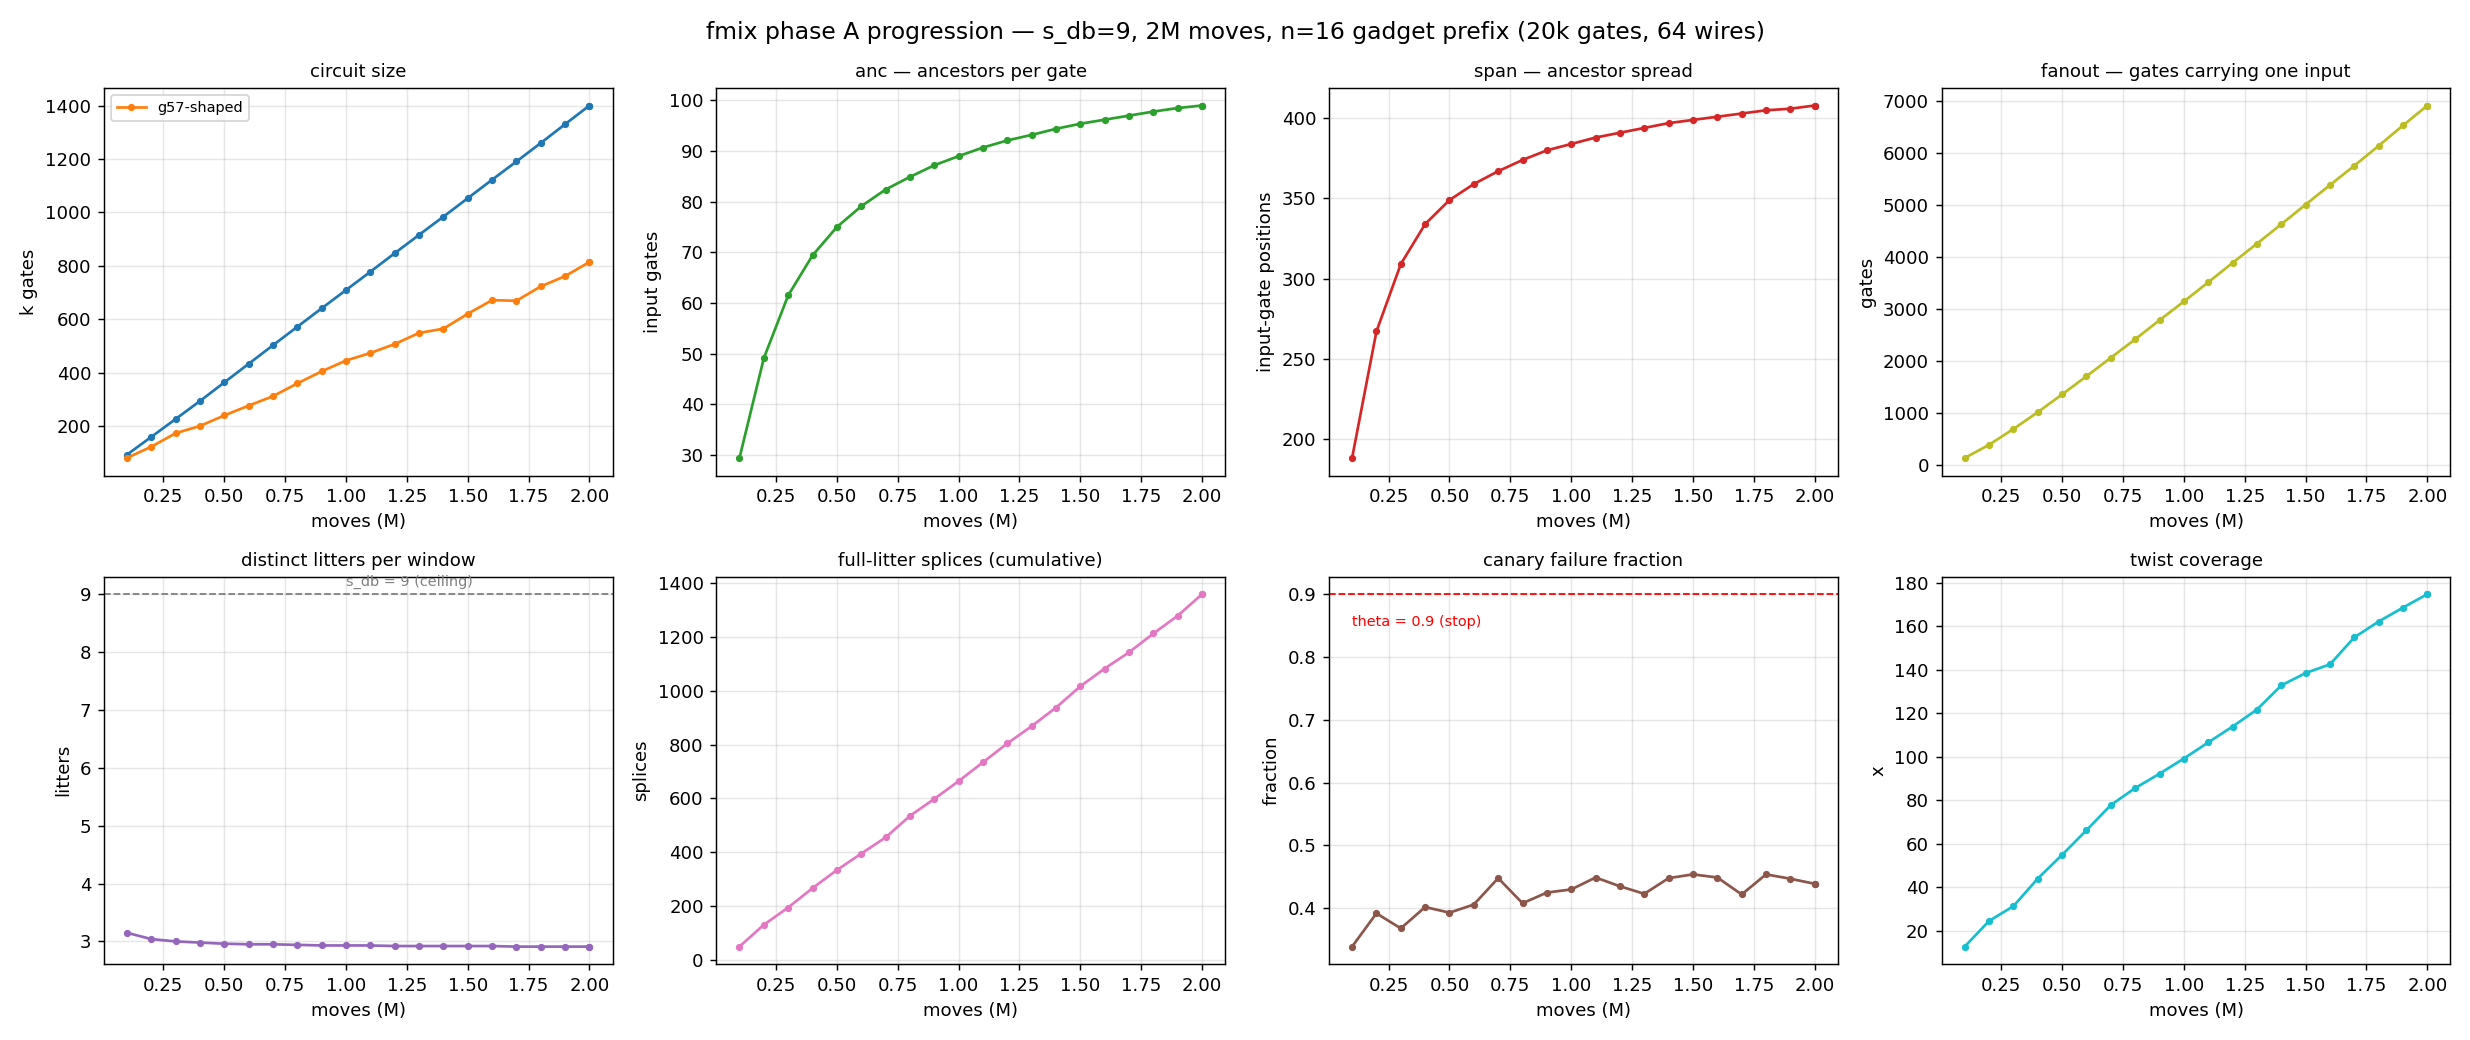
\includegraphics[width=\textwidth]{../reports/ancestry_20260728/prog9b.png}\end{center}

\begin{center}
\begin{tabular}{lrr}
\toprule
& start & 2M \\
\midrule
size & 92k & 1{,}401k \\
\texttt{anc} & 29.4 & 99.0 \\
\texttt{span} & 188 & 408 \\
\texttt{fanout} & 135 & 6{,}909 \\
distinct litters/window & 3.15 & 2.91 \\
canary & 0.339 & 0.439 \\
\texttt{osyn} & 0.983 & \textbf{1.000} \\
\bottomrule
\end{tabular}
\end{center}

Ancestry climbs throughout but decelerates: $\Delta\texttt{anc}$ per 100k falls
from $+32$ to $+0.5$, $\Delta\texttt{span}$ from $+121$ to $+2$, both
approaching an asymptote ($\texttt{anc}\approx 105$, $\texttt{span}\approx 415$).

Litter diversity is flat and low---$3.15\to 2.91$ against a ceiling of
9---and full-litter splices accrue at a dead-constant ${\sim}70$ per 100k moves
from the first interval to the last. That is an equilibrium reached almost
immediately, not a transient: windows keep being drawn from ${\sim}3$
replacement events even though they span 9 gates.

\subsection{Is saturation the input's fault? 10k versus 20k}

\begin{center}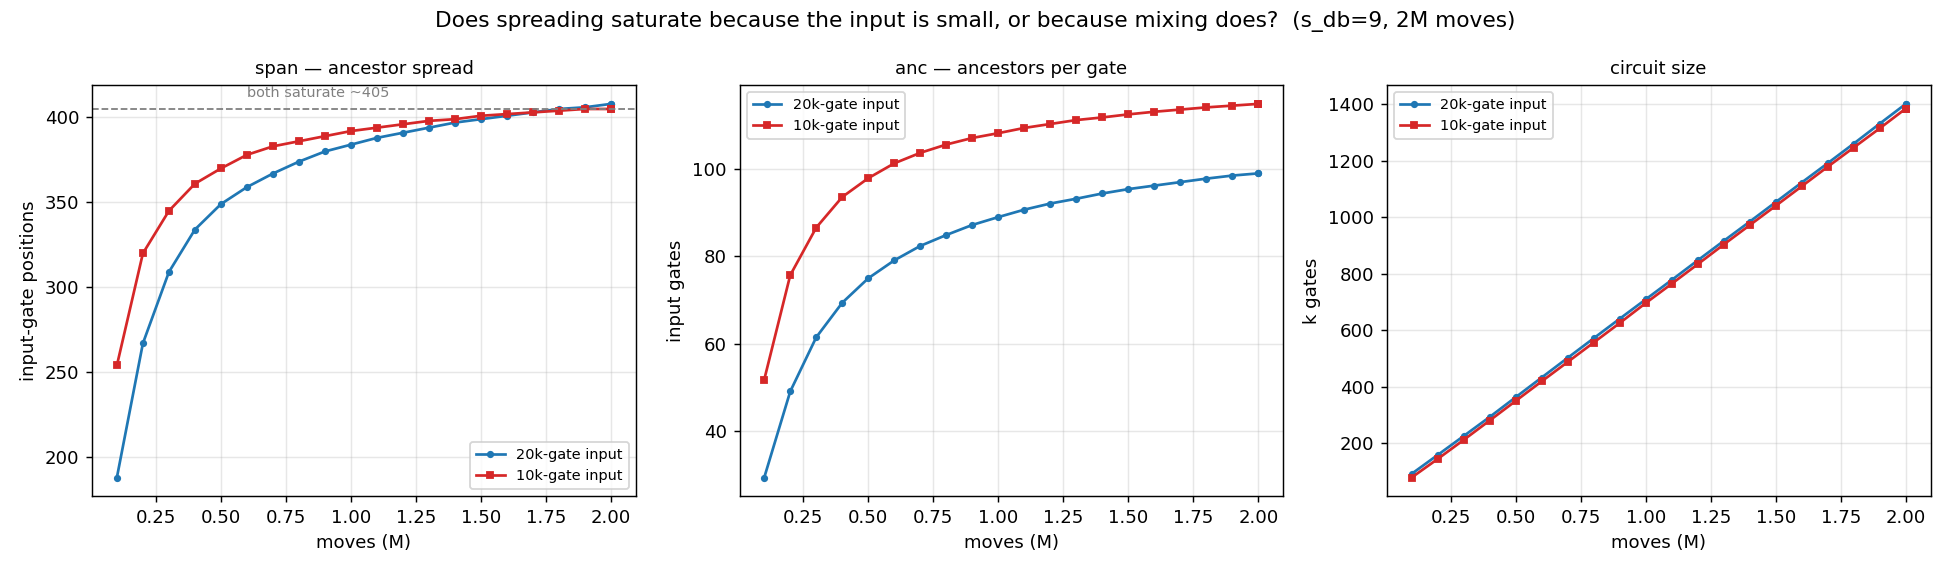
\includegraphics[width=\textwidth]{../reports/ancestry_20260728/input_size_control.png}\end{center}

\begin{center}
\begin{tabular}{lrr}
\toprule
at 2M moves & 20k input & 10k input \\
\midrule
\textbf{span} & \textbf{408} & \textbf{405} \\
\texttt{anc} & 99.0 & 114.9 \\
size & 1{,}401k & 1{,}384k \\
growth ratio & $70\times$ & $\mathbf{138\times}$ \\
\bottomrule
\end{tabular}
\end{center}

Span lands on the same value from a halved input, across runs differing in both
input size and growth ratio. Saturation is a property of the \emph{mixing}, not
a ceiling from the original circuit. \texttt{anc} being higher on the smaller
input fits: same span in absolute positions, but $138\times$ versus $70\times$
growth means more splices per input gate. Growth drives \texttt{anc}; something
else pins \texttt{span}.

\subsection{What pins span: the $s_{db}$ sweep}

\begin{center}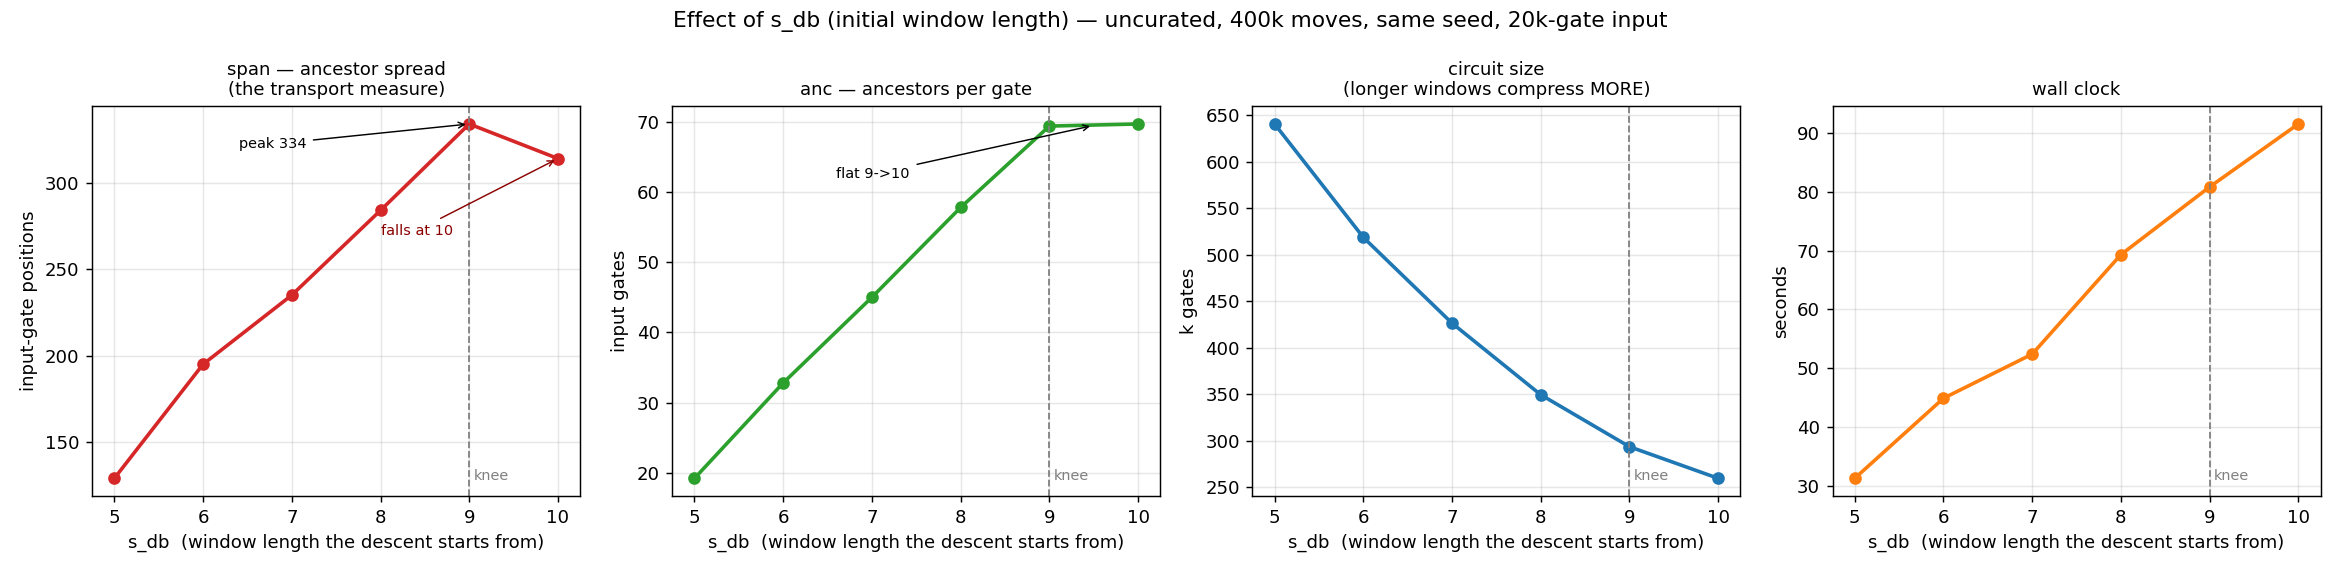
\includegraphics[width=\textwidth]{../reports/ancestry_20260728/sdb_sweep.png}\end{center}

Uncurated, 400k moves, same seed, 20k input.

\begin{center}
\begin{tabular}{rrrrrr}
\toprule
$s_{db}$ & \texttt{anc} & \texttt{span} & \texttt{fanout} & size & wall \\
\midrule
5 & 19.2 & 129 & 614 & 640{,}596 & 31.3\,s \\
6 & 32.8 & 195 & 848 & 518{,}594 & 44.9\,s \\
7 & 45.0 & 235 & 956 & 426{,}263 & 52.4\,s \\
8 & 57.8 & 284 & 1006 & 349{,}262 & 69.3\,s \\
9 & 69.4 & \textbf{334} & 1015 & 293{,}341 & 80.8\,s \\
10 & 69.7 & 314 & 900 & 259{,}335 & 91.5\,s \\
\bottomrule
\end{tabular}
\end{center}

Span rises ${\sim}{+}51$ positions per extra gate of window, then turns at 10;
\texttt{anc} goes flat exactly where span turns ($69.4\to 69.7$)---the same
number of ancestors, packed tighter. So span is a \emph{tunable}, not a limit:
the reach of the mixing operator is set by how much a window spans, and
information travels only as far as overlapping windows carry it. Running longer
buys \texttt{anc}; it buys almost no \texttt{span} after the first ${\sim}500$k
moves.

Size falls 60\% across the sweep and keeps falling past the knee. Longer windows
find free (non-growing) matches far more often---the splice histogram gives the
free fraction as $0/10.5/23.1/39.9/68.8\%$ at lengths 1--5---so they pay less.
Past the knee that extra length is spent on \emph{compression} rather than
combination: the 10-rung behaves like a COMP move embedded in MIX, pulling
toward local minimality. A built-in damper.

\paragraph{Recommendation.} $s_{db}$ of 8--9 rather than the spec's 5:
$3.6\times$ the \texttt{anc}, $2.6\times$ the span, and a circuit $2.2\times$
smaller, for $2.6\times$ the wall clock. The knee should be re-measured on the
$n=128$ gadget, since the store's decay with window length is material-dependent.

\subsection{The exhale: COMP mode}

\begin{center}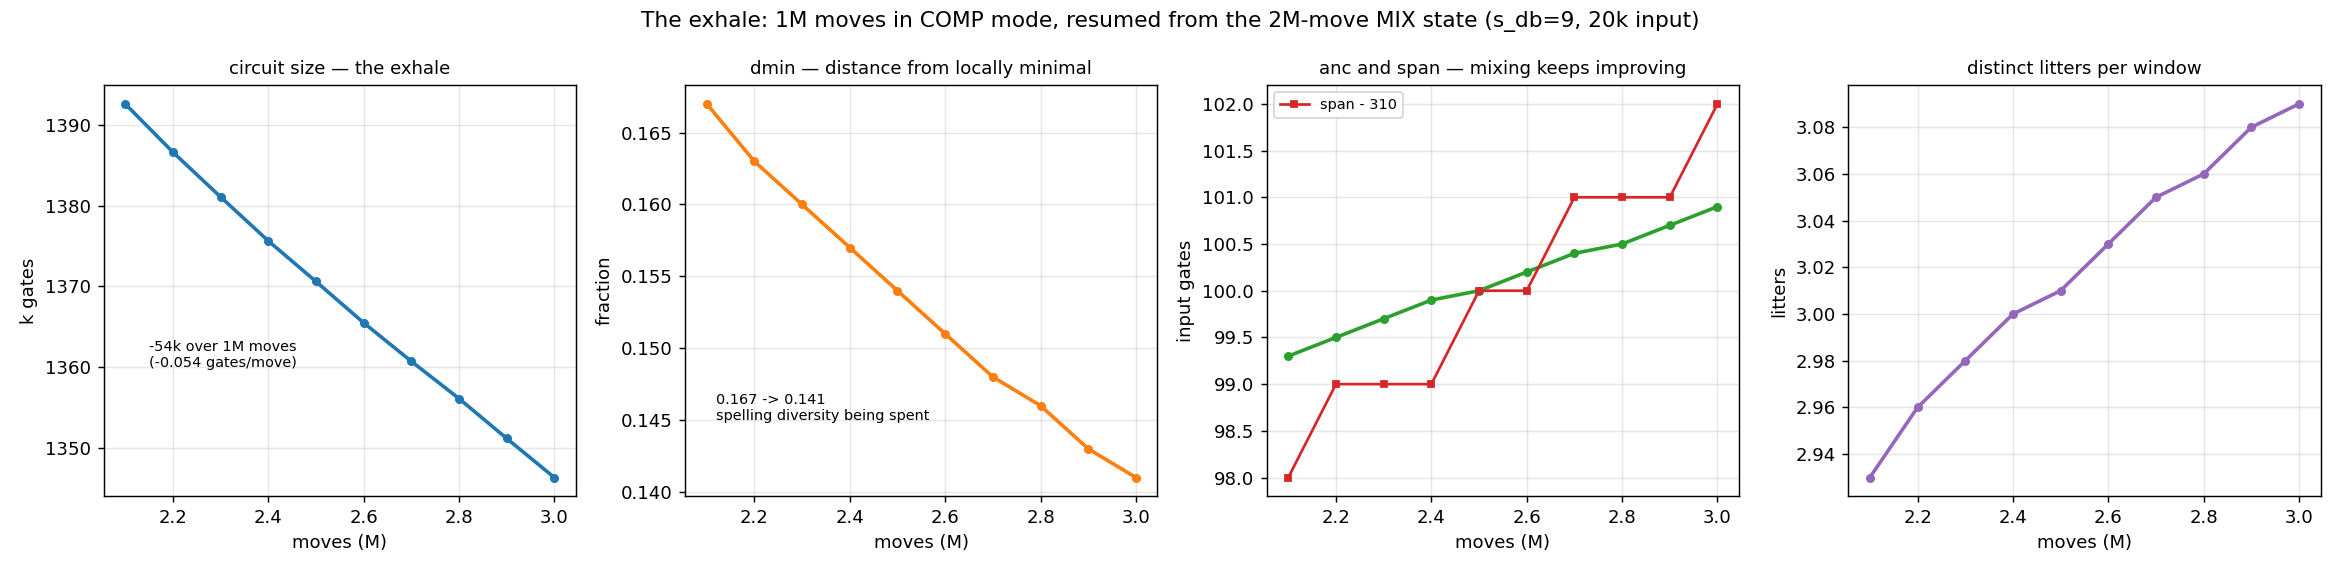
\includegraphics[width=\textwidth]{../reports/ancestry_20260728/exhale.png}\end{center}
\begin{center}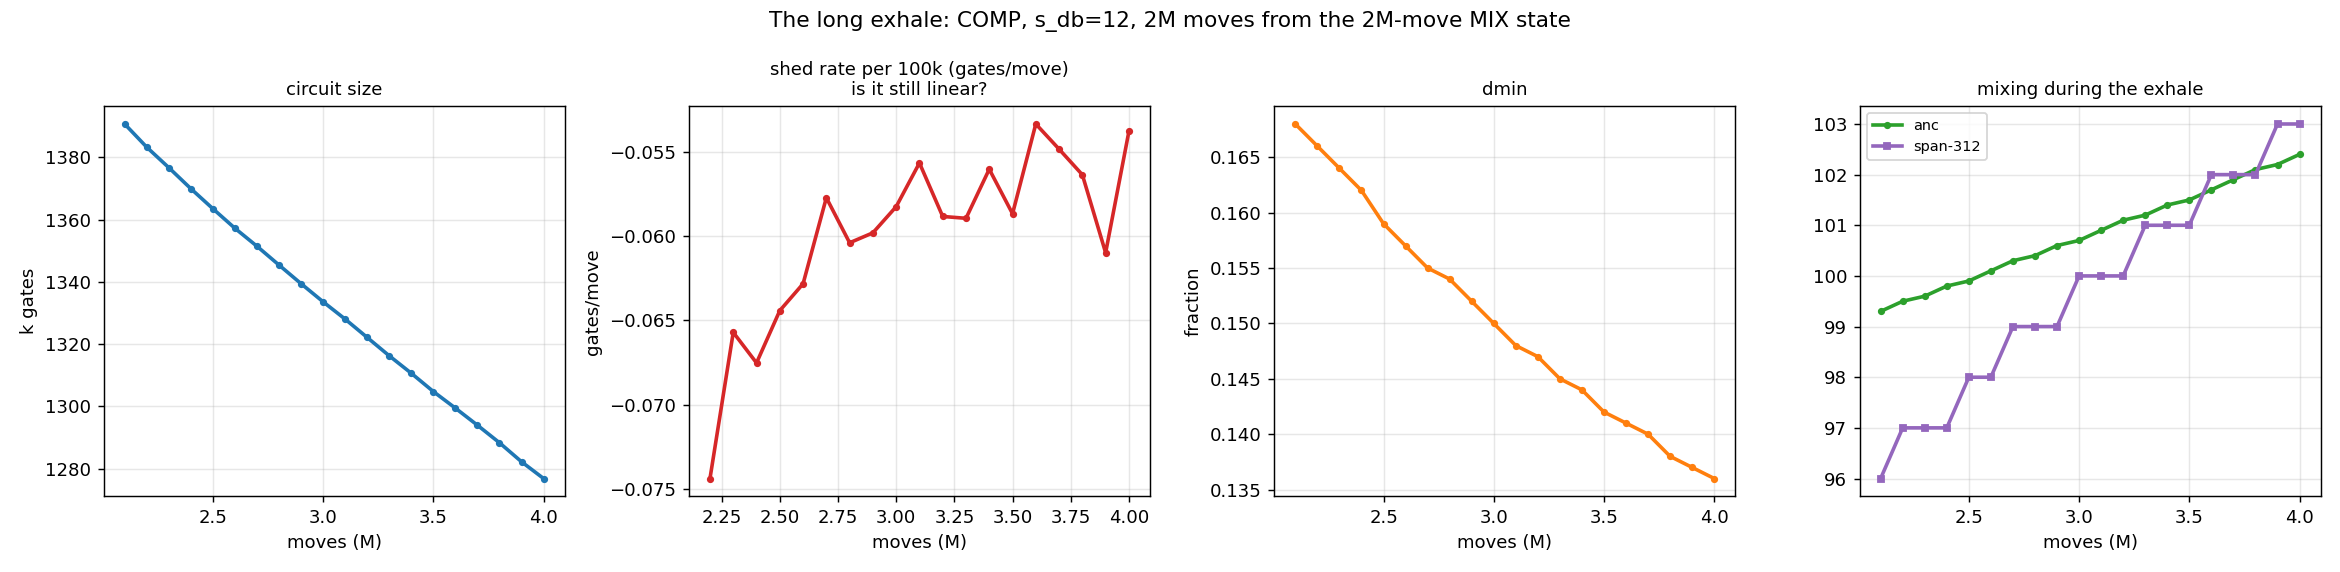
\includegraphics[width=\textwidth]{../reports/ancestry_20260728/comp12.png}\end{center}

\begin{center}
\begin{tabular}{lrr}
\toprule
COMP, $s_{db}=12$, 2M moves & start & end \\
\midrule
size & 1{,}400{,}600 & 1{,}276{,}860 \\
shed rate & $-0.074$ & $-0.056$ (flat) \\
\texttt{dmin} & 0.168 & 0.136 \\
\texttt{anc} & 99.3 & 102.4 \\
\texttt{span} & 408 & 415 \\
distinct litters & 2.97 & \textbf{3.54} \\
\bottomrule
\end{tabular}
\end{center}

COMP wants a longer window than MIX: $-0.060$ gates/move at $s_{db}=12$ against
$-0.054$ at 9, consistent with the sweep, where size kept falling past the
mixing knee.

Mixing does \emph{not} degrade during an exhale. \texttt{anc} and \texttt{span}
both rise, and litter diversity makes its largest move of any run. COMP-DB
splices are still re-encodings---they combine ancestry and stamp
generations---so compression is not idle time.

The cost is entirely in \texttt{dmin}, which falls steadily ($0.168\to 0.136$,
about 19\% of the way to zero) without decelerating: spelling diversity being
spent, the circuit moving toward the locally-minimal form that
\texttt{fcompress}, being attacker-computable, would reach anyway.

No bend appears in 2M moves of exhale---the shed rate decays ${\sim}20\%$ early
then goes flat---so by the ``bend marks the natural inhale point'' criterion
there is a long way still to go.

\section{What this changes}

\begin{enumerate}
\item \texttt{odiff}, \texttt{oadj} and \texttt{disp} should not be quoted
without \texttt{osyn} beside them, and not at all once it is high. Earlier
transport conclusions drawn from them---including ``transport is exactly zero
after $2.58\times$ growth''---are unsupported.
\item \texttt{span} is the transport measure; \texttt{fanout} is \texttt{anc}
times the size ratio and adds nothing; normalised span encodes a target we do
not have.
\item Span saturates for reasons internal to the mixing, and the lever is
window length, not run length.
\item $s_{db}$ should be larger than the spec's 5, with the knee at 8--9 on this
material, and COMP plausibly wanting more than MIX.
\item Litter diversity is the untouched lever: windows draw from ${\sim}3$
replacement events against a ceiling of $s_{db}$, at equilibrium from the start.
\end{enumerate}

\section{Open}

\begin{itemize}
\item Re-measure the $s_{db}$ knee on the $n=128$ gadget (689k gates).
\item Locate the shed-rate bend with a long exhale, and test whether the other
statistics turn at the same point.
\item \texttt{--litter-samples} and \texttt{--litter-ban} are built and untested
against these baselines.
\item Contiguous versus convex sampling has never been separated
($p_{\text{convex}}=0.5$ throughout); COMP and MIX may want different geometry.
\item \texttt{p\_mingen} has been $0.8$ throughout, including in COMP where
weaker pool targeting may serve better.
\item What counts as ``enough'' span needs a reference scale from the
construction, not from the circuit's length.
\end{itemize}

\end{document}
